%; whizzy section -pdf xpdf -latex ./whizzypdfptex.sh
% latex beamer presentation.
% platex, latex-beamer $B$G%3%s%Q%$%k$9$k$3$H$rA[Dj!#(B 

%     Tokyo Debian Meeting resources
%     Copyright (C) 2007 Junichi Uekawa
%     Copyright (C) 2008 Nobuhiro Iwamatsu

%     This program is free software; you can redistribute it and/or modify
%     it under the terms of the GNU General Public License as published by
%     the Free Software Foundation; either version 2 of the License, or
%     (at your option) any later version.

%     This program is distributed in the hope that it will be useful,
%     but WITHOUT ANY WARRANTY; without even the implied warranty of
%     MERCHANTABILITY or FITNESS FOR A PARTICULAR PURPOSE.  See the
%     GNU General Public License for more details.

%     You should have received a copy of the GNU General Public License
%     along with this program; if not, write to the Free Software
%     Foundation, Inc., 51 Franklin St, Fifth Floor, Boston, MA  02110-1301 USA

\documentclass[cjk,dvipdfm,12pt]{beamer}
\usetheme{Tokyo}
\usepackage{ulem}
\usepackage{tabularx}

\usepackage{fancybox}
\usepackage{fancyvrb}   
\usepackage{float}

% commandline$B4D6-$rDj5A!#2hLLF~=PNO$K$D$$$F$O(Bcommandline$B4D6-(B
% $B$GI=5-$9$k(B
\newenvironment{commandline}%
{\VerbatimEnvironment
  \begin{Sbox}\begin{minipage}{1.0\hsize}\begin{fontsize}{7.3}{7.3} \begin{BVerbatim}}%
{\end{BVerbatim}\end{fontsize}\end{minipage}\end{Sbox}
  \setlength{\fboxsep}{8pt}
% start on a new paragraph

\vspace{6pt}% skip before
\fcolorbox{dancerdarkblue}{dancerlightblue}{\TheSbox}

\vspace{6pt}% skip after
}
%end of commandline

\definecolor{dancerdarkblue}{rgb}{0,0.08,0.45}
\definecolor{dancernormalblue}{rgb}{0.8,0.9,0.95}
\definecolor{dancerlightblue}{rgb}{0.8,0.95,1}


%  preview (shell-command (concat "evince " (replace-regexp-in-string "tex$" "pdf"(buffer-file-name)) "&"))
%  presentation (shell-command (concat "xpdf -fullscreen " (replace-regexp-in-string "tex$" "pdf"(buffer-file-name)) "&"))

%http://www.naney.org/diki/dk/hyperref.html
%$BF|K\8l(BEUC$B7O4D6-$N;~(B
\AtBeginDvi{\special{pdf:tounicode EUC-UCS2}}
%$B%7%U%H(BJIS$B7O4D6-$N;~(B
%\AtBeginDvi{\special{pdf:tounicode 90ms-RKSJ-UCS2}}

\title{$BEl5~%(%j%"(B Debian $BJY6/2q(B}
\subtitle{Debian Package $B%O%s%:%*%s(B}
\author{$B4d>>(B $B?.MN(B iwamatsu@debian.or.jp\\IRC nick: iwamatsu}
\date{2008$BG/(B03$B7n(B01$BF|(B}
\logo{
\includegraphics[width=8cm]{image200607/openlogo-light.eps}}


% $B4V$N%?%$%H%k%Z!<%8MQ(B
\newcommand{\emtext}[1]{
\begin{frame}{}
 
\begin{minipage}{0.55\hsize}
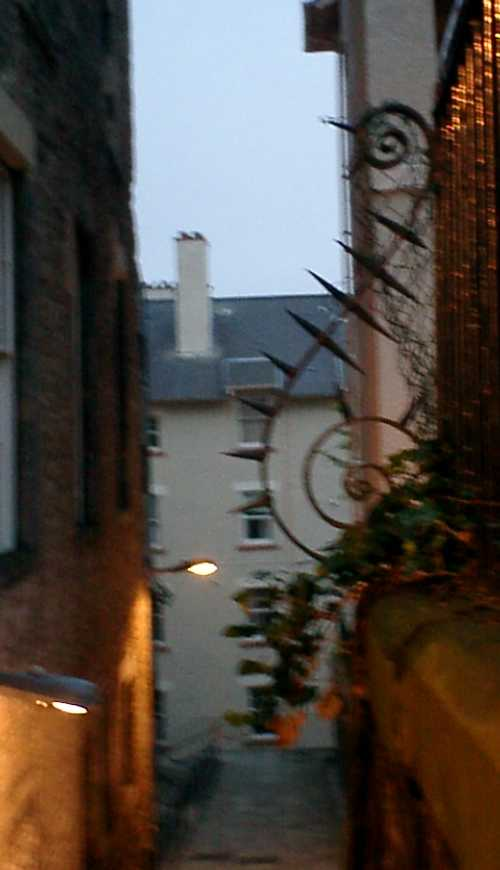
\includegraphics[width=1\hsize]{image200707/gurutitle.jpg}
\end{minipage}
\begin{minipage}{0.39\hsize}
 {\Huge #1
 }
\end{minipage}
\end{frame}
}

\begin{document}
\frame{\titlepage{}}

\section{Intro}

\emtext{Agenda}

\section{}
\begin{frame}
 \frametitle{Agenda}
  \begin{itemize}
  \item $B<+8J>R2p(B
  \item $B:#2s$NL\E*(B
  \item Debian Package $B:n@.4D6-(B
  \item Debian Package $B$r:n@.$9$kA0$N=`Hw(B
  \item Debian Package$B$N?w7A$r:n$k(B
  \item $B%=!<%9%U%!%$%k$NJQ99(B
  \item Debian Package $B$N:n@.(B
  \item $B0MB84X78$N2r7h(B  
  \item $B%Q%C%1!<%8$N%A%'%C%/(B
  \item $B$^$H$a(B
  \item $B<A5?1~Ez(B
 \end{itemize}
\end{frame}

\section{$B<+8J>R2p(B}

\begin{frame}{$B<+8J>R2p(B}
\begin{itemize}
 \item $B4d>>(B $B?.MN!J(BIwamatsu Nobuhiro$B!K(B
 \item Debian JP Project $BI{2qD9(B/Debian Package Maintainer
 \item Linux Kernel / Driver $B$N3+H/$J$I(B
\end{itemize}
\end{frame}

\section{$B:#2s$NL\E*(B}
\emtext{$B:#2s$NL\E*(B}

\begin{frame}
$B%7%s%0%k%P%$%J%j$N(B Debian Package $B$r:n@.$G$-$k$h$&$K$J$k$3$H!#(B
\end{frame}

\section{Debian Package $B:n@.4D6-(B}
\emtext{Debian Package $B:n@.4D6-(B}

\begin{frame}
$B0J2<$N4D6-JQ?t$r@_Dj$7$F$*$/$HJXMx$G$9!#(B

\begin{itemize}
  \item DEBFULLNAME $B$N@_Dj(B

    Debian Pakcage $B$N%a%s%F%JL>(B
  \item DEBEMAIL $B$N@_Dj(B

    Debain Package  $B%a%s%F%J%s%9MQ$N%a!<%k%"%I%l%9(B
\end{itemize}
\end{frame}

\begin{frame}[containsverbatim]

\begin{commandline}
$ cat ~/.bashrc
--$BN,(B-
export DEBFULLNAME="Nobuhiro Iwamatsu"
export DEBEMAIL=iwamatsu@nigauri.org
--$BN,(B--
\end{commandline}

\end{frame}
\begin{frame}{Debian Package $B$N:n@.4D6-(B}
$BI,MW$J%Q%C%1!<%8(B
\begin{itemize}
 \item devscripts
 \item debhelper
 \item lintian/linda
 \item gcc 
 \item binutils 
 \item libc6-dev
\end{itemize}

\end{frame}

\section{$B:#2s$N@8lS(B}
\emtext{$B:#2s$N@8lS(B}

\begin{frame}[containsverbatim]
sl
\begin{commandline}


      ====        ________                ___________
  _D _|  |_______/        \__I_I_____===__|_________|
   |(_)---  |   H\________/ |   |        =|___ ___|      _________________ 
   /     |  |   H  |  |     |   |         ||_| |_||     _|                \_____A
  |      |  |   H  |__--------------------| [___] |   =|                        |
  | ________|___H__/__|_____/[][]~\_______|       |   -|                        |
  |/ |   |-----------I_____I [][] []  D   |=======|____|________________________|_
__/ =| o |=-~~\  /~~\  /~~\  /~~\ ____Y___________|__|__________________________|_
 |/-=|___||    ||    ||    ||    |_____/~\___/          |_D__D__D_|  |_D__D__D_|
  \_/      \__/  \__/  \__/  \__/      \_/               \_/   \_/    \_/   \_/

\end{commandline}
\end{frame}

\section{Debian Package $B$r:n@.$9$kA0$N=`Hw(B}
\emtext{Debian Package $B$r:n@.$9$kA0$N=`Hw(B}


\section{Debian Package $B$N?w7A$r:n$k(B}
\emtext{Debian Package $B$N?w7A$r:n$k(B}

\begin{frame}[containsverbatim]

Debian Package $B$N?w7A$r:n@.$9$k$K$O!"(Bdh\_make $B%3%^%s%I$r;H$$$^$9!#(B
\begin{commandline}
$ mv sl sl-0.0.0
$ cd sl-0.0.0
$ dh\_make 
\end{commandline}
\end{frame}

\begin{frame}[containsverbatim]
\begin{commandline}
iwamatsu@chimagu:~/sl-0.0.0$ dh_make

Type of package: single binary, multiple binary, library, kernel module or cdbs?
 [s/m/l/k/b] 
\end{commandline}
\end{frame}

\begin{frame}
\begin{itemize}
  \item s: single binary
  \item m: multiple binary
  \item l: library
  \item k: kernel module
  \item b: cdbs
\end{itemize}
\end{frame}

\begin{frame}[containsverbatim]
\begin{commandline}
iwamatsu@chimagu:~/sl-0.0.0$ dh_make

Type of package: single binary, multiple binary, library, kernel module or cdbs?
 [s/m/l/k/b] s
Maintainer name : Nobuhiro Iwamatsu
Email-Address   : iwamatsu@nigauri.org 
Date            : Thu, 21 Feb 2008 15:46:57 +0900
Package Name    : sl
Version         : 0.0.0
License         : blank
Type of Package : Single
Hit <enter> to confirm:
\end{commandline}
\end{frame}

\begin{frame}[containsverbatim]
\begin{commandline}
iwamatsu@chimagu:~/sl-0.0.0$ dh_make

Type of package: single binary, multiple binary, library, kernel module or cdbs?
 [s/m/l/k/b] s
Maintainer name : Nobuhiro Iwamatsu
Email-Address   : iwamatsu@nigauri.org 
Date            : Thu, 21 Feb 2008 15:46:57 +0900
Package Name    : sl
Version         : 0.0.0
License         : blank
Type of Package : Single
Hit <enter> to confirm:
 
Could not find sl_0.0.0.orig.tar.gz
Either specify an alternate file to use with -f,
or add --createorig to create one.
\end{commandline}
\end{frame}

\begin{frame}[containsverbatim]
xxx.orig.tar.gz $B$,$J$$$H!"%(%i!<$K$J$j$^$9!#(B\\
--createorig $B%*%W%7%g%s$r2C$($F!!(Bdh\_make$B$r<B9T$7$^$9!#(B

\begin{commandline}
$ dh_make --createorig
\end{commandline} 
\end{frame}

\section{}

\begin{frame}[containsverbatim]

dh\_make $B<B9T8e!"(Bdebian $B%G%#%l%/%H%j$,:n@.$5$l$^$9!#(B
\begin{commandline}
README.Debian  control    dirs    emacsen-remove.ex   
init.d.lsb.ex  manpage.xml.ex     mogeri.doc-base.EX  
preinst.ex     watch.ex$B!!!!!!!!!!!!(B    changelog  copyright  
docs           emacsen-startup.ex manpage.1.ex     
menu.ex        postinst.ex        prerm.ex
compat         cron.d.ex          emacsen-install.ex  
init.d.ex      manpage.sgml.ex    sl-default.ex  
postrm.ex      rules
\end{commandline}
*.ex / *.EX $B$O%5%s%W%k$J$N$G!":o=|$7$^$9!#(B

\end{frame}

\begin{frame}[containsverbatim]

$B:GDc8BI,MWL>%U%!%$%k$O0J2<$NDL$j$G$9!#(B
\begin{itemize}
  \item README.Debian --$B!!(BPackage $B$N(BREADME
  \item control       -- Package $B$N@bL@!"%S%k%I$KI,MW$J>pJs$J$I(B
  \item dirs          -- Package $B$GMxMQ$9$k%G%#%l%/%H%j$r5-=R(B
  \item changelog     -- Package $B$NJQ99MzNr(B
  \item copyright     -- Package $B$N%3%T!<%i%$%H(B
  \item docs          -- $B%I%-%e%a%s%H(B
  \item rules         -- Package $B:n@.MQ$N%9%/%j%W%H(B(Makefile)
  \item compat
\end{itemize}
\end{frame}


\section{$B$H$j$"$($:(B Package $B$r:n@.$9$k(B}
\emtext{$B$H$j$"$($:(B Package $B$r:n@.$9$k(B}
\begin{frame}[containsverbatim]
\begin{commandline}
$ debuild -us -uc
\end{commandline}
\end{frame}
\begin{frame}


Makefile $B$NJT=8(B
install:
clean:
distclean:
$B!!(BDESTDIR $B$N@bL@(B

Debian Package $B$N:n@.(B
 debuild 
  $B0l2sL\$G%(%i!<%3%s%Q%$%k%(%i!<$,=P$k$N$,M}A[(B
 $B0MB84X78$N2r7h(B
 lintian / linda

 $B%Q%C%1!<%8:n@.;~$N%(%i!<$r=$@5(B

\end{frame}

\section{Debian Package$B$N%F%9%H(B}
\emtext{Debian Package $B$N%F%9%H(B}

\section{}
\begin{frame}
\begin{itemize}
  \item pbuilder

   $B:GDc8B$N(BDebian system $B$+$i!"%Q%C%1!<%8$r:n@.$9$k$?$a$N%D!<%k!#(B 

  \item piuparts 

   Debian Package $B$N(B $B%$%s%9%H!<%k(B/$B%"%s%$%s%9%H!<%k$N%A%'%C%/$r$9$k$?$a$N%D!<%k!#(B

\end{itemize}
\end{frame}

\section{$B$^$H$a(B}
\emtext{$BK\F|$N$^$H$a(B}

\section{}
\begin{frame}
\begin{itemize}
  \item dh\_make $B$G%Q%C%1!<%8$N?w7A$r:n@.(B
  \item debuild $B$G%Q%C%1!<%8:n@.(B
  \item lintian/linda $B$G(B $B%Q%C%1!<%8$N%A%'%C%/(B
  \item $B%$%s%9%H!<%k$7$FF0:n3NG'$^$G9T$&(B
  \item $B%"%s%$%s%9%H!<%k$N3NG'$bK:$l$:$K(B
\end{itemize}
\end{frame}

\section{$B=*$o$j$K(B}
\emtext{$B=*$o$j$K(B}

\section{}
\begin{frame}
$B:#G/$N(BDebian$BJY6/2q$G$O!"Kh7nMM!9$J(BDebian Pakcage $B$N(B
$B:n@.J}K!$r$_$J$5$s$KEA<x$7$^$9!#(B
\begin{itemize}
  \item $B%G!<%?$@$1$N(BDebianPackage$B:n@.J}K!(B
  \item VCS$B$r;H$C$?(BDebian Package$B$N:n@.J}K!(B
  \item $B%i%$%V%i%j$N(BDebian Package $B:n@.J}K!(B
  \item $B$J$I$J$I(B
\end{itemize}
\end{frame}


\section{$B<A5?1~Ez(B}
\emtext{$B<A5?1~Ez(B}

\end{document}

;;; Local Variables: ***
;;; outline-regexp: "\\([ 	]*\\\\\\(documentstyle\\|documentclass\\|emtext\\|section\\|begin{frame}\\)\\*?[ 	]*[[{]\\|[]+\\)" ***
;;; End: ***
